\documentclass[12pt,letterpaper]{beamer}
\usetheme{Copenhagen}
\usecolortheme{seahorse}
\setbeamertemplate{section in toc}{\inserttocsection}

\usepackage[utf8]{inputenc}
\usepackage{amsmath}
\usepackage{amsfonts}
\usepackage{amssymb}
\usepackage{graphicx}
\graphicspath{ {./images/} }
\usepackage{multirow}
\usepackage{hyperref}
\hypersetup{
    colorlinks=true,
    linkcolor=blue,
    filecolor=magenta,      
    urlcolor=cyan,
    pdftitle={Overleaf Example},
    pdfpagemode=FullScreen,
}
\usepackage{minted}

\title[Robotics I]
{ENGR 3421: ROBOTICS I}
\subtitle{ArUco}

\author[Zhang, Lin]
{Dr. Lin Zhang}
\institute[UCA] % (optional)
{
  Department of Physics and Astronomy\\
  University of Central Arkansas
}
\date[Robotics1 2021] % (optional)
{September 21, 2021}
\logo{
\includegraphics[height=1cm]{../images/uca_bear_logo.png}}


%End of title page configuration block
%------------------------------------------------------------

%------------------------------------------------------------
%The next block of commands puts the table of contents at the beginning of each section and highlights the current section:

% \AtBeginSection[]
% {
  % \begin{frame}
    % \frametitle{Outline}
    % \tableofcontents[currentsection]
  % \end{frame}
% }
%------------------------------------------------------------

\begin{document}

%The next statement creates the title page.
\frame{\titlepage}

%---------------------------------------------------------
%This block of code is for the table of contents after the title page
% \begin{frame}
% \frametitle{Outline}
% \tableofcontents
% \end{frame}
%---------------------------------------------------------


\begin{frame}[fragile]
\frametitle{Install OpenCV}

Install OpenCV for Python if you only want to detect the markers:
{\scriptsize
    \begin{minted}{bash}
sudo apt install python3-opencv
    \end{minted}
}

To get the latest OpenCV in Python, so that you can access more updated features:
{\scriptsize
    \begin{minted}{bash}
pip3 install opencv-contrib-python numpy --upgrade
sudo apt-get install -y libatlas-base-dev \
libhdf5-dev \
libhdf5-serial-dev \
libatlas-base-dev \
libjasper-dev \
libqtgui4 \
libqt4-test
# optional, install matplotlib
sudo apt install python3-gi-cairo
pip3 install matplotlib
    \end{minted}
}
\end{frame}

\begin{frame}{ArUco Marker}
    \begin{columns}
        \column{0.5\textwidth}
        An ArUco marker is a synthetic square marker composed by a wide black border and a inner binary matrix which determines its identifier (id). 
        {\scriptsize
            \begin{itemize}
                \item Camera calibration
                \item Object size estimation
                \item Measuring distance
                \item 3D pose estimation
            \end{itemize}
        }
        Refer to \href{https://docs.opencv.org/4.5.2/d5/dae/tutorial_aruco_detection.html}{OpenCV's tutorial}.
        \column{0.5\textwidth}
        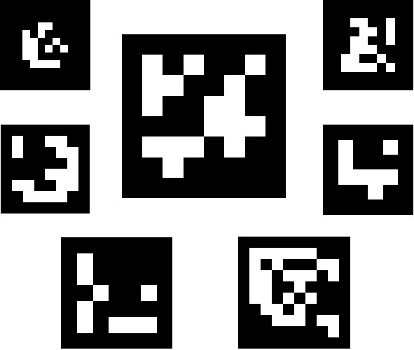
\includegraphics[width=0.8\linewidth]{aruco_markers}
    \end{columns}
\end{frame}

\begin{frame}{Markers and Dictionaries}

    $cv2.aruco.DICT\_NXN\_M$
    {\scriptsize
        \begin{itemize}
            \item The dictionary size, $M$, is the number of markers that compose the dictionary. 
            \item The marker size , $N$, is the size of those markers (the number of bits).
            \item Smaller $M$ and $N$ are preferable.
            \item Higher-quality input images are preferable.
        \end{itemize}
    }

\end{frame}

\begin{frame}[fragile]
    \frametitle{Marker Creation}

    {\scriptsize
    \begin{minted}{python}
import cv2
import numpy as np
import matplotlib.pyplot as plt

dictionary = cv2.aruco.Dictionary_get(cv2.aruco.DICT_4X4_50)
id = 23
resolution = 300
output_array = np.zeros((300, 300, 1), dtype="uint8")
border_size = 1
marker = cv2.aruco.drawMarker(
    dictionary, 
    id, 
    resolution, 
    output_array, 
    border_size
)

plt.imshow(marker)
plt.show()
    \end{minted}
}
\end{frame}

\begin{frame}{Marker Detection}

    Each detected marker includes:
    {\scriptsize
        \begin{itemize}
            \item The position of its four corners in the image (in their original order).
            \item The id of the marker.
        \end{itemize}
    }
    Marker detection process:
    {\scriptsize
        \begin{enumerate}
            \item Detection of marker candidates
            \item Determine if they are actually markers by analyzing their inner codification.
        \end{enumerate}
    }
\end{frame}

\begin{frame}[fragile]
    \frametitle{Marker Detection}
    \scriptsize
    \begin{minted}{python}
import cv2

arucoDict = cv2.aruco.Dictionary_get(cv2.aruco.DICT_4X4_50)
arucoParams = cv2.aruco.DetectorParameters_create()

vid = cv2.VideoCapture(0)
while True:
    ret, img = vid.read()
    (corners, ids, rejects) = cv2.aruco.detectMarkers(
        img,
        arucoDict,
        parameters=arucoParams
    )
    cv2.aruco.drawDetectedMarkers(
        image=img,
        corners=corners,
        ids=ids
    )
    cv2.imshow("detection", img)
    if cv2.waitKey(1) == ord("q"):
        break

vid.release()
cv2.destroyAllWindows()
    \end{minted}
\end{frame}

\end{document}

